\documentclass[11pt,letterpaper,oneside]{report}
\usepackage{url}
\usepackage{hyperref}
% margenes del documento
\usepackage[letterpaper,top=3.5cm,left=3.5cm,bottom=2.5cm, right=2.5cm]{geometry}
% numeración de páginas a la derecha
\usepackage{fancyhdr}
\pagestyle{fancy}
\fancyhf{}
\renewcommand{\headrulewidth}{0pt}
\renewcommand{\footrulewidth}{0pt}
\rfoot{\thepage}
% cuadros de la portada
\usepackage{xcolor}
\usepackage{framed}
\definecolor{shadecolor}{rgb}{0,0,0}
% espacio entre lineas
\renewcommand{\baselinestretch}{1.5}
% letra Arial
\usepackage{helvet}
\renewcommand{\familydefault}{\sfdefault}
% cambiar estilo del capítulo
\usepackage{titlesec}
% sangría
\setlength{\parindent}{0cm}
% codificacion
\usepackage[utf8]{inputenc}
% lenguaje
\usepackage[spanish,es-tabla]{babel}
% punto decimal     				
\spanishdecimal{.} 
% matematicas y simbolos             				
\usepackage{amsmath,amssymb}
% url
\usepackage{url}
% graficas y subfiguras
\usepackage{graphicx, subfigure}
%\usepackage{morefloats} 	% Más figuras
%\usepackage[section]{placeins} 	% Figs en sección
%\usepackage{endfloats} 	% Figs al final
\newenvironment{proof}[1][Demostración]{\textbf{#1.} }{\
  \hfill \rule{0.5em}{0.5em}}
% conteo consecutivo de figuras y tablas
\usepackage{chngcntr}
\counterwithout{equation}{chapter}
\counterwithout{figure}{chapter}
\counterwithout{table}{chapter}
% numeros romanos para tablas
\renewcommand{\thetable}{\Roman{table}} 		% Roman for tables
% definición de entornos
\newtheorem{define}{Definición}
\newtheorem{proposition}{Proposición}
\newtheorem{theorem}{Teorema}
\newtheorem{lemma}{Lema}
\newtheorem{remark}{Observación}
\newtheorem{property}{Propiedad}
% división de palabras
\hyphenation{}
\pagenumbering{roman}
%%%%%%%%%%%%%%%%%%%%%%%%%%%%%%%%%%%%%%%%%%%%%%%%%%%%%%%%%%%%%%%%%%%%%%%%%%%%%%%%%%%%%%%%%%%%%%%%%%%%
\begin{document}
%%%%%%%%%%%%%%%%%%%%%%%%%%%%%%%%%%%%%%%%%%%%%%%%%%%%%%%%%%%%%%%%%%%%%%%%%%%%%%%%%%%%%%%%%%%%%%%%%%%%
\renewcommand{\contentsname}{ÍNDICE}
\renewcommand{\listfigurename}{LISTA DE FIGURAS}
\renewcommand{\listtablename}{LISTA DE TABLAS}
\renewcommand{\bibname}{BIBLIOGRAFÍA}
\thispagestyle{empty}
\begin{figure}[!t]
\centering

\includegraphics[width=0.55\textwidth, height=0.25\textheight]{./figs/logoclr}
\end{figure}

\begin{center}

{\bf \LARGE ``Diseño de un coprocesador para la operación de la convolución con Verilog en FPGA''}

\vspace*{0.75cm}

{\bf \Large Tesis }

\vspace*{0.65cm}

{\Large que para el obtener el título de}

\vspace{0.65cm}

{\bf \Large ``Ingeniero en Electrónica''}

\vspace{0.75cm}

\begin{framed}

{\large Presenta:}

\vspace{0.3cm}

{\large Roberto Emmanuel Valenzuela Armenta}

\vspace{0.3cm}

{\large Asesor:}

\vspace{0.3cm}

{\large Dr. Eduardo Romero Aguirre}

\end{framed}

\vfill

\begin{shaded*}
{\large {\color{white}Ciudad Obregón, Sonora \hfill \today}}
\end{shaded*}

\end{center}

\pagebreak
\newpage
\thispagestyle{empty}

\vspace*{5cm}
\hfill \emph{No obstante, un matemático, que reforzara su profecía con fórmulas y terminologías matemáticas, podría no ser comprendido por nadie y, sin embargo, creído por todos.}

\bigskip
\hfill \emph{Isaac Asimov, Preludio a la Fundación}

\pagebreak
\newpage
\thispagestyle{empty}

\begin{center}
{\bf \Large AGRADECIMIENTOS}
\end{center}

\vspace*{1cm}

Agradezco principalmente a mi familia que por su esfuerzo estoy aquí terminando una etapa de mi vida y me dieron la oportunidad de estudiar esta carrera.\\

A los amigos que hice a lo largo de la carrera, que viví experiencias con ellos y nos ayudamos los unos a los otros a completar nuestros logros en los proyectos y trabajos.\\


\pagebreak
\newpage
%\thispagestyle{empty}

\begin{center}
{\bf \Large RESUMEN}
\end{center}

\vspace{1cm}

El siguiente proyecto se realiza con el fin de realizar un simulador utilizando herramientas de software libre para el curso tradicional de robótica a nivel licenciatura para ello se realiza una investigación de trabajos previos con el fin de conocer los distintos softwares que se han hecho anteriormente. Con la información recaudada se logra crear un diseño de un manipulador de 3 grados de libertad en V-Realm Builder y un panel de control el cual se piensa añadir al funcionamiento del manipulador para futuras interacciones.


%%%%%%%%%%%%%%%%%%%%%%%%%%%%%%%%%%%%%%%%%%%%%%%%%%%%%%%%%%%%%%%%%%%%%%%%%%%%%%%%%%%%%%%%%%%%%%%%%%%%
\titleformat{\chapter}{\centering\normalfont\Large\bfseries}{\thechapter}{1em}{}
\thispagestyle{fancy}
%\listoffigures
{%
\let\oldnumberline\numberline%
\renewcommand{\numberline}{\figurename~\oldnumberline}%
\listoffigures
}
\thispagestyle{fancy}
%\listoftables
{%
\let\oldnumberline\numberline%
\renewcommand{\numberline}{\tablename~\oldnumberline}%
\listoftables
}
\thispagestyle{fancy}
\tableofcontents
\titleformat{\chapter}{\vspace{0.5\textheight}\centering\normalfont\Large\bfseries}{\thechapter}{1em}{}
%%%%%%%%%%%%%%%%%%%%%%%%%%%%%%%%%%%%%%%%%%%%%%%%%%%%%%%%%%%%%%%%%%%%%%%%%%%%%%%%%%%%%%%%%%%%%%%%%%%%
\renewcommand\thechapter{\Roman{chapter}}
\chapter{INTRODUCCIÓN} \label{ch:intro} \thispagestyle{fancy} \pagenumbering{arabic}
\renewcommand\thechapter{\arabic{chapter}}
%%%%%%%%%%%%%%%%%%%%%%%%%%%%%%%%%%%%%%%%%%%%%%%%%%%%%%%%%%%%%%%%%%%%%%%%%%%%
% trabajo cuenta con un diseño y desarrollo un laboratorio virtual el cual maneja un brazo robótico con el fin de que el usuario pueda interactuar y reforzar los conceptos básicos que se ven en el curso de robótica de nivel licenciatura. Es una herramienta la cual se enfoca en la ''enseñanza para la comprensión'', hoy en día los simuladores se vuelven mejor con las tecnologías que nos rodean, se pueden crear software el cual maneje mejor ciertos parámetros para asemejarse mas a la realidad que nos rodea y no necesitar de equipos caros, se busca igualar la manera de trabajar aunque no se tenga físicamente, pero que se sienta que la interacción es la misma.

%---------------------------------------------------------------------------------------
\section{Antecedentes}
Los simuladores surgen por la necesidad de crear sistemas de apoyo para el usuario ya sea aprendiendo de manera práctica, realizando descubrimientos, situaciones hipotéticas o simples pruebas de laboratorio aprovechando las especificaciones de la computadora para poder recrear dichas acciones visualizándolas de la mejor manera.\\

Hoy en día hay una infinidad de simuladores como análisis estadísticos, construcción, circuitos electrónicos, juegos y éstos ayudan a que las tareas sean más sencillas o que la teoría pueda aterrizarse de manera práctica de tal forma que se combinan muchas habilidades como el aprender a usar dicho programa, visualizar la manera en que se comporta la simulación y la aplicación de ésta misma; nos ayudan a evitar que ocurra un problema a la hora de aplicar el trabajo realizado esto es un factor importante, es evidente entonces que nos ahorra el tener que reparar un equipo en caso de que no haya funcionado, se observa claramente que otro punto es el hecho de hacernos saber si el proyecto es viable o no. En \cite{moran-2009} mencionan ''enseñanza para la comprensión'' que facilita el conocer los conceptos básicos de los robots creando una herramienta didáctica para ayudar en la comprensión de la teoría y logren obtener buenas bases sobres los conceptos manejados y las aplicaciones que tiene la robótica.\\

Existen formas las cuales pueden facilitar como lo son las pruebas físicas sin tener un equipo de una gran cantidad monetaria, se menciona en \cite{berenguel-2016} y \cite{lancheros-2010} que con piezas Lego$\copyright$  fueron capaces de realizar tele-robots mediante un software y un sistema electrónico el cual permitía aprender de una manera didáctica la forma en la que se comportaban los movimientos de dicho robot.\\

En la Universidad de Alicante \cite{pomares-2004} nos habla del impacto que tienen los laboratorios virtuales en los alumnos, dice que un 90\% de los alumnos necesita menos de 1 hora para poder comprender el simulador, mientras que a un 46\% le basta con 30 minutos, solo al 15\% les ha faltado tiempo para realizar la práctica propuesta con una duración máxima de 2 horas. Muestran gráficas las cuales concluyen que el 10\% de los alumnos necesitan más de 2 horas para poder comprender mejor el simulador, mientras que el 5\% lo dominan. Además, explican que muchos de los alumnos están conformes con trabajar vía simulación y desde casa ya que algunos asisten a la escuela y trabajan, pero el laboratorio virtual beneficia en el ámbito que les facilita el traslado y prefieren estar trabajando en su casa, por otra parte, el 71\% de los alumnos menciona que prefiere hacerlo en la escuela por las dudas que puedan surgir a la hora de estar haciendo las prácticas de dicho laboratorio.\\

En el libro \cite{selman-2002} nos habla de como el lenguaje de Java es uno de los cuales puede trasladarse de manera sencilla, el hecho de poder crear un código con una aplicación, ésta la podemos llevar ya sea en el celular, en la web, una PC con Windows, Mac OS o linux. La API de Java3D ofrece mucho al desarrollador, así como al definir objetos para elementos tales como apariencias, transformaciones, materiales, luces, etc.\\

El mundo de la robótica es caro, pero lo bueno es que existen programas alternos los cuales permiten crear, testear y simular de estos productos; Gazebo$\copyright$ \cite{gazebo-2014} es un simulador el cual permite al usuario usar un robot existente, modificar el mismo y adaptarle sensores para la aplicación final que se desee, es en tiempo real dicho lo anterior el poder usar sensores se encuentra dentro de los plugins del mismo programa ya que estos son las librerías con las cuales se pueden complementar el proyecto a realizar, la comunicación el ambiente de trabajo del robot, etc. Por otro lado, existe Coppelia Robotics$\copyright$ el cual cuenta con virtual robot experimentation platform (V-rep$\copyright$) es un programa portable ya que se puede manejar en Windows, Mac OS y linux.

\section{Definición del problema}
Como ejemplo tenemos que en las instituciones tratan siempre de tener tecnologías para los alumnos, equipos con los cuales puedan interactuar y aprender, pero en ciertas ocasiones existen impedimentos que los detienen para brindar ese servicio ya sea que el precio es muy elevado o que consideran que no vale la pena invertir para que solo tenga una aplicación básica y no se haga uso de todas las capacidades que éste tendría. En la clase de robótica el alumno muy difícilmente podría entender los conceptos teóricos, aunque estén todas las características de este, simplemente llevando a la práctica la teoría hay mas probabilidades de comprensión. 

¿Se puede realizar un simulador utilizando herramientas de software libre para el curso tradicional de robótica a nivel licenciatura?

\section{Justificación}
Un aspecto importante en la ingeniería es que a la hora de estar estudiando la teoría hay veces que se aterriza mejor esos conocimientos de manera práctica; Los laboratorios son importantes, es donde se aplican los conocimientos teóricos, pero no todos cuentan con equipos necesarios, ya que algunos pueden llegar a ser caros, por eso se busca que el usuario pueda interactuar por medio de estas herramientas y poder realizar acciones que complementen su clase para que comprenda mejor sus conocimientos, sin tener que tener un equipo físicamente, basta con un simulador que cumpla las características.

\section{Objetivos}
Diseñar y desarrollar un laboratorio virtual de robótica de manipuladores mediante la integración de gráficos vectorizados, cálculo simbólico y Java 3D con el fin de proporcionar una herramienta que fortalezca el proceso enseñanza-aprendizaje en el curso de robótica industrial.

\section{Hipótesis}
\begin{itemize}
\item Utilizar un software el cual permita diseñar en 3D un brazo robótico. 
\item Mediante Java3D poder recrear el diseño de Solidworks para que el usuario interactúe.
\end{itemize}

\section{Delimitaciones}
\begin{itemize}
\item El contenido aquí mencionado no se llevará a la práctica por lo que no se obtendrá una estadística para finalmente saber el impacto que este tendría. Es decir, no se probará el alcance de comprensión de la persona que se queda con los conceptos básicos de la clase y otra que adquiere conceptos de manera experimental en dicho laboratorio.
\item Se realizará un diseño en específico de un robot con 6 Grados De Libertad (GDL), esto indica que no podrá abarcar todos los posibles escenarios, distintas variantes de robots o de movimientos.
\end{itemize}

\section{Limitaciones}
\begin{itemize}
\item Debido a la falta de tiempo solo se llevará a cabo la implementación de la cinemática.
\end{itemize}

\renewcommand\thechapter{\Roman{chapter}}
\chapter{MARCO TEÓRICO} \label{ch:marco} \thispagestyle{fancy}
\renewcommand\thechapter{\arabic{chapter}}
%%%%%%%%%%%%%%%%%%%%%%%%%%%%%%%%%%%%%%%%%%%%%%%%%%%%%%%%%%%%%%%%%%%%%%%%%%%%
En la robótica un manipulador es una herramienta que ayuda a controlar objetos sin necesidad de hacer contacto directo \cite{ARQHYS-2012}; consisten en una secuencia de cuerpos rígidos llamados eslabones, se conectan unos con otros mediante articulaciones formando una cadena cinemática. Se dice que una cadena cinemática es abierta si, numerando de manera secuencial los eslabones desde el primero, cada eslabón está conectado mediante articulaciones exclusivamente al eslabón anterior, y al siguiente, excepto el primero, que se suele fijar al suelo, y el último, uno de cuyos extremos queda libre.

\begin{figure}
\centering
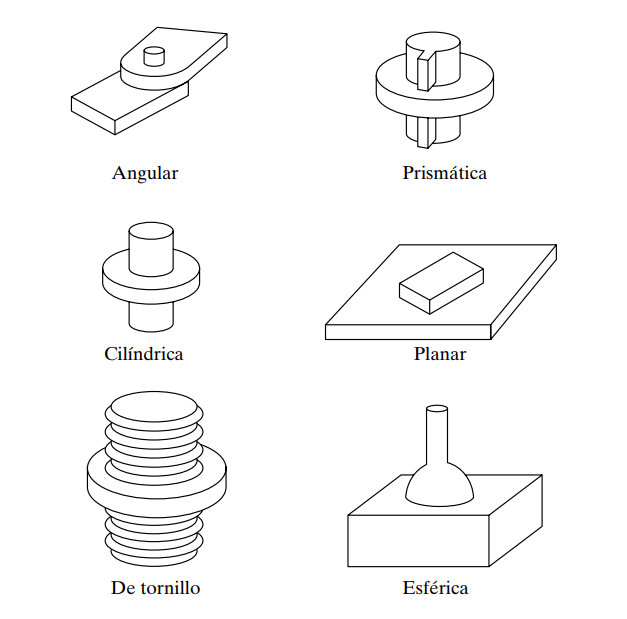
\includegraphics[width=0.5\textwidth, height=0.375\textheight]{./figs/6Articulaciones}
\caption{Tipos de mecanismos}
\label{mecanismos}
\end{figure}

Los movimientos que pueden realizar cada articulación de manera independiente se le denomina grado de libertad (GDL).
\begin{itemize}
\item La articulación angular permite que dos eslabones giren, uno respecto del otro, alrededor del eje de articulación; tiene 1 GDL.
\item La articulación prismática permite que dos eslabones arreglados en pares se deslicen, uno respecto al otro a lo largo de su eje; tiene 1 GDL.
\item La articulación cilíndrica permite la rotación alrededor del eje de la articulación y el traslado independiente a lo largo de ella; tiene 2 GDL.
\item La articulación plana permite dos traslados a lo largo de dos ejes independientes del plano de contacto y una rotación alrededor del eje perpendicular del plano.
\item La articulación de tornillo permite que dos eslabones unidos giren alrededor del eje de la articulación y se trasladen, al mismo tiempo, a lo largo de él; consta de 1 GDL.
\item La articulación esférica permite que uno de los eslabones pareados gire libremente en todas las orientaciones posibles respecto al otro alrededor del centro de una esfera; tiene 3 GDL.\\
\end{itemize}

\textbf{Grado de libertad}\\
Formalmente un grado de libertad de un sistema mecánico se define como el número de coordenadas mínimas necesarias para describir perfectamente su posición o configuración. Así, un cuerpo rígido que se mueve en el espacio cartesiano tridimensional tiene seis GDL, tres para posición y tres para orientación.\\ 

\textbf{Cinemática de los robots}\\
La cinemática es un derivado de la física que estudia el movimiento sin considerar las fuerzas o pares que lo causan, es decir, estudia las leyes de movimiento sin tener en cuenta aspectos como masas e inercias. Estudia la trayectoria que tiene el robot a lo largo del tiempo, considerando la posición, velocidad y en ocasiones la aceleración. En otras palabras se puede decir que describe de manera analítica el movimiento espacial del robot como una función del tiempo.\\

\textbf{Cinemática Directa}\\
Se le conoce como a los modelos matemáticos que permiten calcular la posición de los eslabones de un robot a partir de sus componentes fijos y configuraciones de las articulaciones.\\
Se refiere al uso de ecuaciones para el cálculo de la posición del actuador final en un robot articulado a partir de los ángulos y/o desplazamientos de las articulaciones o de la posición y orientación de las bases de un robot móvil a partir de las velocidades de las ruedas.\\

\begin{figure}[!h]
\centering
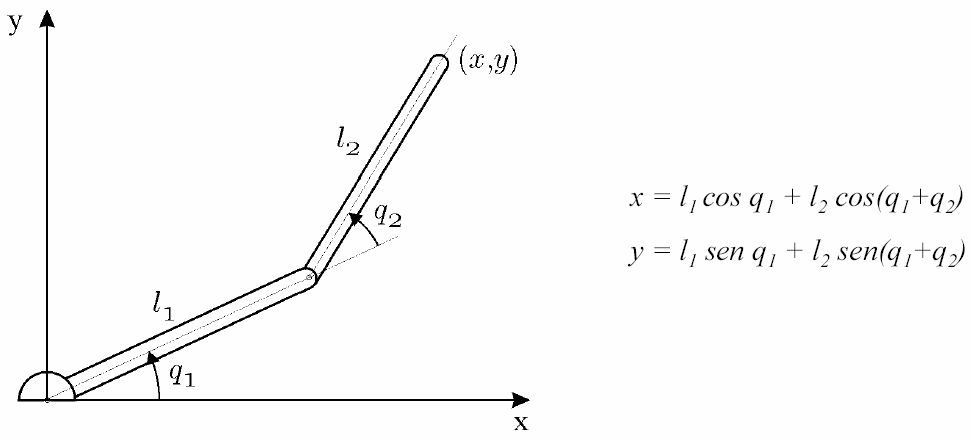
\includegraphics[width=0.7\textwidth, height=0.25\textheight]{./figs/robot2GDL_cinematica_directa}
\caption{Robot de 2GDL}
\label{robot2gdl}
\end{figure}

\newpage
\textbf{Cinemática Inversa}\\
Es el proceso inverso por el cual se obtienen modelos matemáticos que permiten, a partir de una posición y/o desplazamientos de los actuadores. Por lo general podemos encontrar configuraciones que no son factibles, es decir, que no son alcanzables, soluciones múltiples, ya sea que el robot ejerza un movimiento con codo hacia arriba o con codo hacia abajo.

\begin{figure}[!h]
\centering
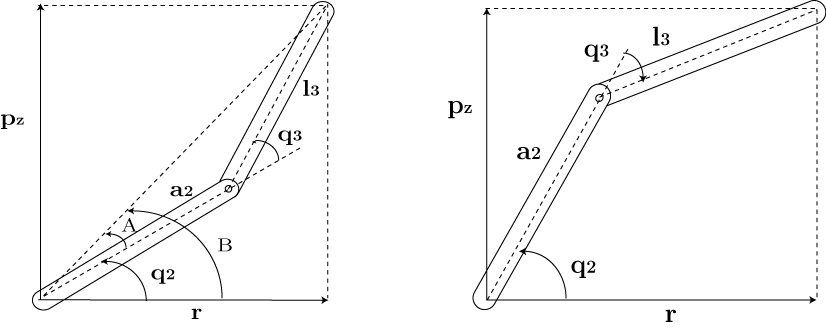
\includegraphics[width=0.8\textwidth, height=0.27\textheight]{./figs/codoarribaabajo}
\caption{Codo hacia abajo y hacia arriba}
\label{codos}
\end{figure}

Los problemas de la cinemática inversa suelen usar métodos aproximados para el cálculo de las variables de articulación, por ejemplo, a partir de la pseudo-inversa de la matriz Jacobiano. Para el caso de un robot articulado con 6GDL, la solución exacta pasa por desacoplar los tres primeros ejes de los tres últimos. En este sentido, la posición del efector final determina los valores de los tres primeros ejes, mientras que la orientación del efector final determina los valores de las tres últimas articulaciones.\\

\textbf{Metodología de Denavit-Hartenberg}\\
La metodología de Denavit-Hartenberg (D-H) permite establecer la ubicación de los sistemas de referencia de los eslabones en los sistemas robóticos articulados, ya sean prismáticas o de revolución, con cadenas cinemáticas abiertas. Jacques Denavit y Richard Hartenberg introdujeron esta convención en 1955 con el propósito de estandarizar la ubicación de los sistemas de referencia de los eslabones de un robot.\\

\newpage
\textbf{Parámetros D-H}\\
Se trata de una metodología ampliamente utilizada en el ámbito académico y de investigación en robótica que permite definir las transformaciones relativas entre eslabones con tan solo cuatro parámetros siento éste el número mínimo de parámetros para configuraciones genéricas.\\


La metodología de D-H define cuatro transformaciones que se aplican de forma consecutiva.
\begin{itemize}
\item d: Desplazamiento a lo largo de z anterior a la normal común.
\item $\theta$: Ángulo sobre la z anterior, de la x anterior a la nueva x.
\item l: Longitud de la normal común. Suponiendo una articulación revoluta, este es el radio de z anterior.
\item $\alpha$: Ángulo sobre la normal común, del antiguo eje z al nuevo eje z.
\end{itemize}

El contenido anterior fue obtenido del libro de \textit{Introducción a la robótica} \cite{saha-2010} de Subir Kumar Saha y de \textit{Fundamentos de la robótica} \cite{barrientos-2007} de A. Barrientos, L. Peñin, C. Balaguer, R. Aracil.\\

\textbf{SolidWorks}\\
SolidWorks es un programa de diseño que consiste en la especificación de puntos, líneas, curvas o superficies a través de un conjunto de parámetros iniciales y de las relaciones existentes entre ellos. Para el diseño, el modelado paramétrico es un recurso muy importante ya que proporciona ventajas como reducir el tiempo y esfuerzo que se requieren al modificar y realizar variaciones en éste y elimina tareas repetitivas al realizar variantes en el diseño.\\

En el programa se crean tres tipos de archivos: piezas, ensambles y dibujo. Además estos archivos están relacionados entre sí, es decir, cuando se realiza la modificación del dibujo, ésta afecta automáticamente a todos los archivos donde se encuentra referenciada la pieza realizada. \cite{herrera-2016} \\

\newpage
\textbf{MatLab}\\
MATLAB es una de las muchas sofisticadas herramientas de computación disponibles en el comercio para resolver problemas de matemáticas, tales como Maple, Mathematica y MathCad. Cada una permitirá efectuar cálculos matemáticos básicos, pero difieren en el modo como manejan los cálculos simbólicos y procesos matemáticos más complicados, como la manipulación de matrices. Por ejemplo, MATLAB es superior en los cálculos que involucran matrices, mientras que Maple lo supera en los cálculos simbólicos. El nombre mismo de MATLAB es una abreviatura de Matrix Laboratory, laboratorio matricial. En un nivel fundamental, se puede pensar que estos programas son sofisticadas calculadoras con base en una computadora. Son capaces de realizar las mismas funciones que una calculadora científica, y muchas más.\\
En muchas clases de ingeniería, la realización de cálculos con un programa de computación matemático como MATLAB sustituye la programación de computadoras más tradicional. MATLAB se han convertido en una herramienta estándar para ingenieros y científicos. \cite{moore-2007}\\

\textbf{Simulink}\\
Simulink® 3D Animation ™ proporciona aplicaciones para vincular modelos Simulink y algoritmos MATLAB® a objetos gráficos 3D. Los objetos se pueden representar en los lenguajes de modelado 3D estándar X3D y VRML97. Puede animar un mundo tridimensional cambiando la posición, la rotación, la escala y otras propiedades del objeto durante el escritorio o la simulación en tiempo real. También puede detectar colisiones y otros eventos en el mundo virtual y alimentarlos de nuevo en sus algoritmos de MATLAB y Simulink. El video de las cámaras virtuales se puede transmitir a Simulink para su procesamiento.

Simulink 3D Animation incluye editores y visualizadores para renderizar e interactuar con escenas virtuales. Con 3D World Editor, puede importar formatos de archivos CAD y URDF, así como crear escenas detalladas ensambladas a partir de objetos 3D. El mundo 3D se puede ver de forma inmersiva con la visión estereoscópica. Puede incorporar múltiples vistas de escena en 3D dentro de las figuras de MATLAB e interactuar con el mundo virtual usando un joystick de retroalimentación forzada, un mouse espacial u otro dispositivo de hardware. \cite{mathw-2018} \\

\textbf{Java 3D}\\
Java 3D es una interfaz de programación de aplicaciones (API) desarrollada en Sun Microsystems para renderizar gráficos 3D interactivos utilizando el lenguaje de programación Java. Java 3D es una API de Java del lado del cliente. Otros ejemplos de API del lado del cliente de Sun incluyen Abstract Windows Toolkit (AWT) y Java Foundation Classes (JFC / Swing), que son ambas bibliotecas de clases Java para crear aplicaciones con una Interfaz gráfica de usuario (GUI). Las API de Java del lado del cliente contrastan con las API del lado del servidor de Sun tales como Enterprise Java-Beans (EJB) y los otros componentes de Java 2 Enterprise Edition (J2EE). 

La principal ventaja de los desarrolladores de Java 3D para Java es que les permite programar en Java al 100 por ciento. En cualquier aplicación 3D grande, el código de representación solo constituirá una fracción de la aplicación total. Por lo tanto, es muy atractivo tener código de aplicación, persistencia y código de interfaz de usuario (UI) en un lenguaje fácilmente portátil, como Java. \cite{selman-2002}\\

Megan Flanders \cite{flanders-2015} menciona que la realidad virtual está jugando un papel muy importante como herramienta educacional que hace mas tangible los conceptos para los estudiantes; concuerdo totalmente ya que una vez vistos los conceptos es mas sencillo aplicarlos en un programa y observar como se comportan de manera visual, además que se aprende a utilizar un software, se fortalece la teoría aplicándola de manera práctica en un programa.\\
En su artículo se observa que el menú es amigable con el usuario, fácil de interpretar y modificar las opciones para poder visualizar los resultados finales ya dentro del mismo simulador. Es la idea tomar en cuenta que como va orientado para alumnos, ellos tienen que comprender de la mejor manera los resultados arrojados por el mismo programa para que capten la teoría utilizando el software.\\
Se muestran resultados por parte de los alumnos ya que se realizaron encuestas los cuales mayormente el 55\% dicen que la herramienta sería una gran parte complementaria al curso, además el 61\% comenta que es fácil de usar el 61\% menciona que es mas fácil entender de manera interactiva con modelos en 3D que con dibujos en 2D, además se muestra que el 74\% comenta que ha incrementado ligeramente su conocimiento en estos temas.\\
Build-a-robot fue creado con MatLab y sus herramientas de VRLM para poder tener los modelos 3D. MatLab contiene muchas herramientas que facilitan a los ingenieros el poder simular, crear y desarrollar ideas, ya que cuenta con herramientas dentro del mismo programa que son complementarias y como corren dentro del mismo es mas sencillo tener acceso y combinarlas para poder crear un buen proyecto.\\

En el artículo de P. Abreu \cite{abreu-2015} habla sobre un laboratorio virtual a diferencia de lo que se quiere realizar este va enfocado a la industria, se tiene el mismo objetivo que es crear un simulador solo que este toma en cuenta además del robot maquinaria con la cual se desea trabajar, se simula el ambiente en el cual el robot estará operando y se puede llegar a una conclusión de si será optimo usar al robot para dicha etapa de producción o a lo que se requiera llevar a cabo. RobotStudio tiene un menú algo mas complicado en el aspecto que a comparación del de Megan y lo que se desea hacer este tiene un teach pendant y un distinto ambiente virtual, está lleno de símbolos, muestra la pantalla del teach pendan y los diferentes menús para poder utilizar el simulador, toman diferentes caminos, como se ha mencionado está hecho para un ambiente más robusto que enfoca otras características.

\renewcommand\thechapter{\Roman{chapter}}
\chapter{MÉTODO} \label{ch:metodo} \thispagestyle{fancy}
\renewcommand\thechapter{\arabic{chapter}}
%%%%%%%%%%%%%%%%%%%%%%%%%%%%%%%%%%%%%%%%%%%%%%%%%%%%%%%%%%%%%%%%%%%%%%%%%%%%
En este capítulo se describe la ruta metodológica que se tomó para diseñar y desarrollar el coprocesador para la convolución. Primero, se indica el sujeto de estudio. Después, se muestra un diagrama de flujo con las etapas del proyecto, así como la descripción de cada una. Por último, se enlistan los materiales y herramientas utilizados.


\section{Sujeto}
\begin{itemize}
\item Investigadores e ingenieros del area de desarrollo de hardware y cómputo de alto rendimiento. 
\end{itemize}

\section{Procedimiento}

\begin{figure}[!h]
\centering
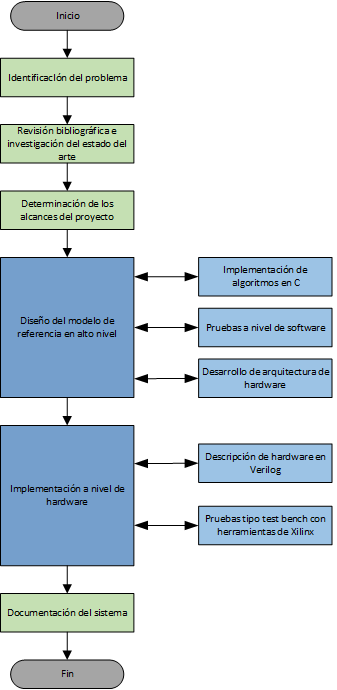
\includegraphics[width=1\textwidth, height=1\textheight]{./figs/procedimiento}\\
\caption{Diagrama de flujo}
\label{diagramaflujo}
\end{figure}

\newpage
En la figura \ref{diagramaflujo} se muestran los pasos que se siguieron para desarrollar el coprocesador para la convolución. A continuación, se describre cada una de las etapas del proyecto.

\subsection{Identificación del problema e investigación}
Se determina la problemática, en base al análisis del entorno actual de la computación, al cual se le buscará solución con el proyecto que se presenta en este trabajo. El problema que se aborda es la necesidad de encontrar alternativas a las tendencias actuales para el procesamiento de señales con mejores prestaciones de cómputo intensivo y con menor consumo de potencia, específicamente para la operación de la convolución.

Además, se recopila información acerca de trabajos similares en bases de datos de artículos científicos y en libros técnicos. Esta información sirve como punto de referencia para comparar el rendimiento de la arquitectura propuesta en este trabajo, además se analizan las áreas de oportunidades de estos trabajos para proponer una solución más óptima al problema planteado. En esta etapa se investiga cuál es la situación actual de la tecnología de cómputo de alto rendimiento la cual se describe en el estado del arte.

\subsection{Determinación de los requerimientos y alcances del proyecto}
Se determinan los requerimientos que se buscan satisfacer con el coprocesador desarrollado en este trabajo. Además, se indican cuáles son los alcances y delimitaciones del proyecto. Este trabajo se limitará a diseñar  la arquitectura de un coprocesador capaz de resolver la operación de la convolución de dos señales. Se implementará en un FPGA y se verificará a través de un entorno de simulación con la ayuda de MATLAB, donde se realizarán pruebas de rendimiento con respecto al tiempo de procesamiento. Las limitaciones del proyecto son el tiempo disponible, dinero, recursos y licencias.

\subsection{Programación en MATLAB de algoritmos de convolución}
Se programan diferentes algoritmos existentes para resolver la convolución utilizando MATLAB. El objetivo de esta etapa es comparar el rendimiento en tiempo de ejecución y uso de recursos de memoria de los diferentes algoritmos y analizar las ventajas y desventajas de cada uno de ellos. 

\subsection{Desarrollo de la arquitectura mediante herramientas de software}
Se desarrolla la arquitectura en un ambiente de software, haciendo uso de programas de software para descripción y simulación de la arquitectura, una metodología de diseño y un lenguaje de descripción de hardware. 

\subsubsection{Diseño de la arquitectura}
Mediante el uso de la metodología Top-Down y en base a las arquitecturas de la actualidad se desarrolla una arquitectura capaz de realizar la operación de la convolución con un menor consumo de potencia y con una velocidad de procesamiento comparable con las arquitecturas modernas.  

\subsubsection{Desarrollo de arquitectura con Verilog}
Con la ayuda de un lenguaje de descripción de hardware, en este caso Verilog, se describe la arquitectura digital en Xilinx ISE 14.7. Se describen los diferentes bloques que forman parte de la arquitectura, posteriormente se unen estos elementos con un top level para formar un sistema capaz de convolucionar dos señales.

\subsubsection{Pruebas - validación funcional}
Se simula la arquitectura mediante el uso de test benchs. Los resultados se comparan con resultados obtenidos con la función predeterminada de MATLAB llamada conv() la cual realiza la operación de la convolución de dos señales. En caso de no obtener los resultados esperados, se vuelve a diseñar la arquitectura. 

\subsubsection{Síntesis}
Se realiza la síntesis lógica del código, la cual consiste en convertir la descripción de hardware especificada mediante Verilog en una implementación de diseño en término de compuertas lógicas, la cual es un archivo de flujo de bits (.bit).  

\subsection{Implementación a nivel de hardware}
En esta etapa se programa el FPGA. Además, se realizan pruebas a la arquitectura propuesta para comprobar que se cumplen los requerimientos planteados al inicio del proyecto y para verificar que la operación de la convolución se realiza de manera correcta. 

\subsubsection{Implementación en FPGA}
Una vez que se cuenta con la arquitectura sintetizada, se programa el archivo de flujo de bits en el FPGA utilizando el software Digilent Adept. Este archivo le indica al FPGA cómo se tiene que configurar para realizar la operación de la convolución.

\subsubsection{Pruebas}
Se realizan pruebas al hardware mediante una interfaz de comunicación serial la cual conecta al FPGA con una PC. Se envian dos señales al FPGA, las cuales se convolucionan en la arquitectura digital, y este da como resultado una tercera señal la cual se envía a la PC. El resultado se compara con resultados obtenidos bajo un ambiente conocido en MATLAB y sirve para comprobar que el sistema digital está funcionando de manera correcta. Además, se realizan pruebas de velocidad de procesamiento y consumo de potencia para comparar con diferentes arquitecturas.

\subsection{Documentación}
Por último, se realiza un trabajo escrito en el cual se documentan los aspectos más relevantes del proyecto. Primero, se da una introducción al proyecto y se pone en contexto al lector, después se presenta el trabajo realizado así como se describe a detalle la forma en que se realizó cada etapa, posteriormente, se presentan los resultados obtenidos así como un análisis de los mismos, haciendo una comparación con las arquitecturas que ya están disponibles en el mercado, por último, se concluye y se proponen mejoras para trabajos futuros. 

\section{Materiales y Herramientas}
\begin{itemize}
\item Laptop Dell Inspiron 13-5378
\item MathWorks MATLAB R2015a
\item Xilinx ISE 14.7
\item Digilent Adept
\color{red}
\item agregar los que faltan (FPGA, OS(?))
\end{itemize}

\renewcommand\thechapter{\Roman{chapter}}
\chapter{DESARROLLO} \label{ch:desarrollo} \thispagestyle{fancy}
\renewcommand\thechapter{\arabic{chapter}}
%%%%%%%%%%%%%%%%%%%%%%%%%%%%%%%%%%%%%%%%%%%%%%%%%%%%%%%%%%%%%%%%%%%%%%%%%%%%
En este capítulo se describe el desarrollo del diseño para la implementación del laboratorio virtual. Se muestra el diagrama de flujo a seguir para llevar a cabo la programación y como es que va a funcionar. Finalmente se presenta la etapa que se esta siguiendo, con un robot de 3GDL el cual es realizar un simulador básico para poder comprender las características que se debe de tener.

\newpage
\begin{figure}[!h]
\centering
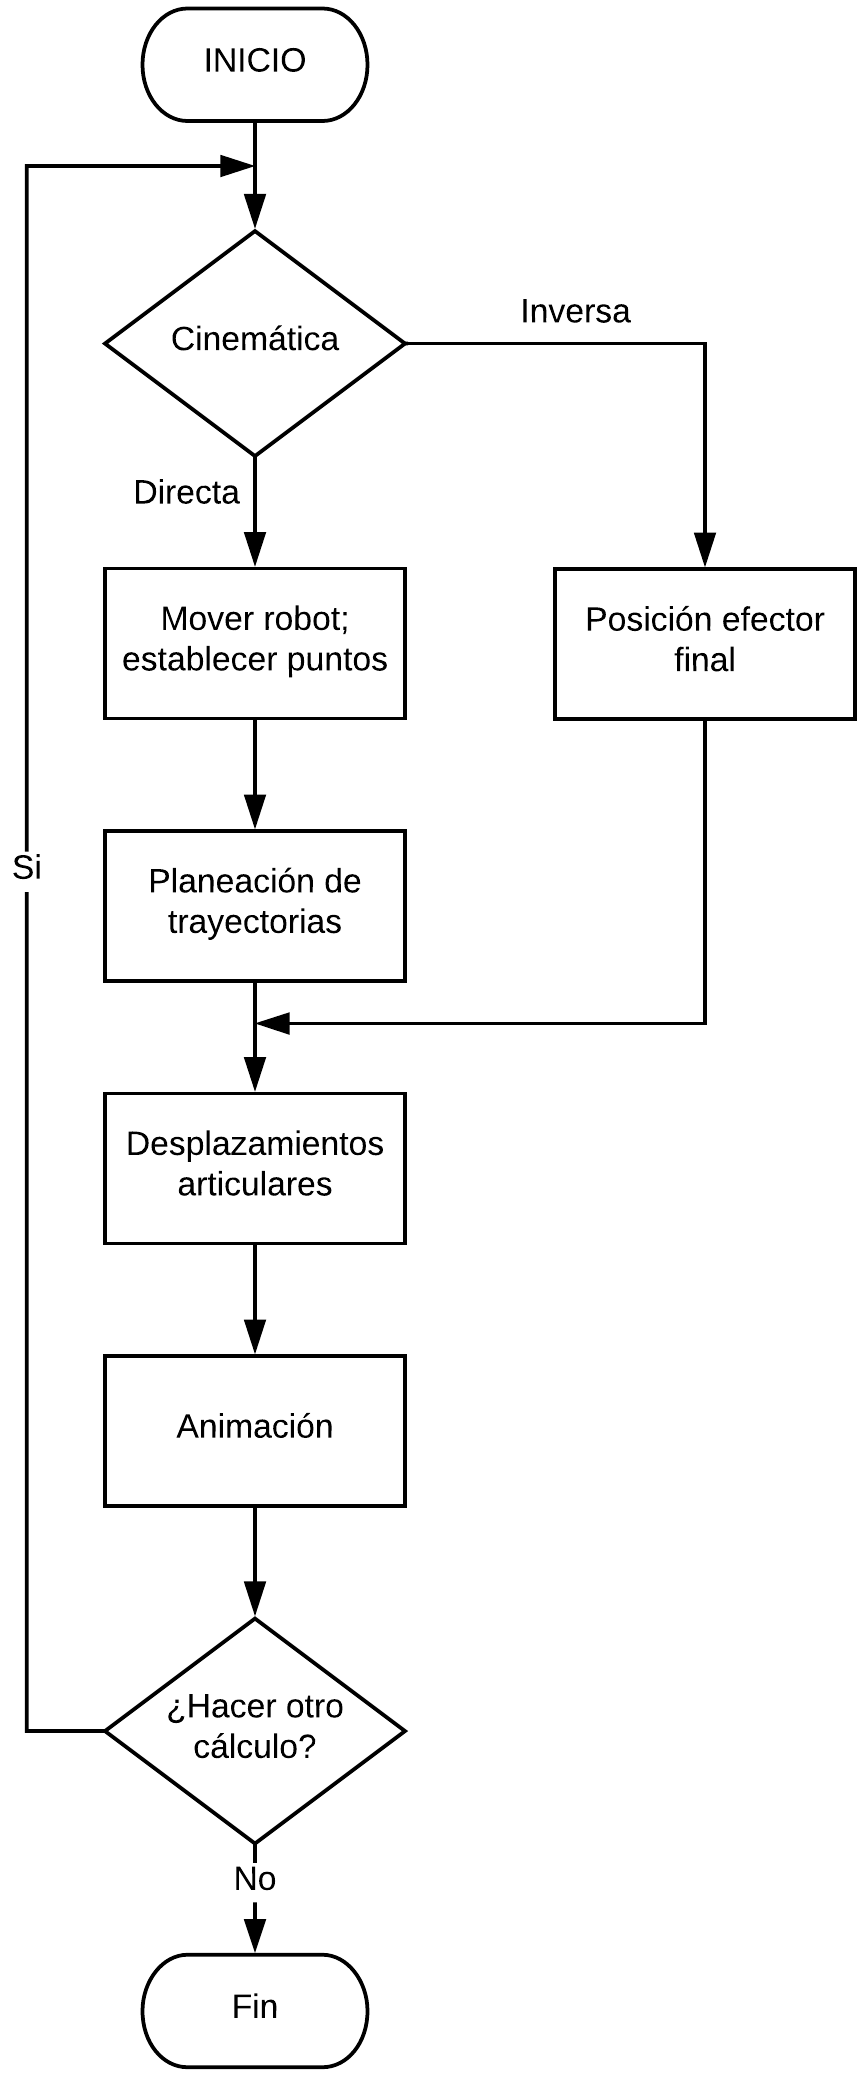
\includegraphics[width=0.45\textwidth, height=0.75\textheight]{./figs/diagramaprogramacion}\\
\caption{Diagrama de flujo para la programación}
\label{diagramadeprogramacion}
\end{figure}

En la figura \ref{diagramadeprogramacion} se quiere iniciar con un menú el cual despliegue dos simples opciones, una la cual va a llevar al cálculo de la cinemática directa y otro de la cinemática inversa, según la opción que se seleccione en este caso si fue la directa se mostrará un menú el cual permita posicionar las articulaciones de manera libre, a continuación realizará una planeación de trayectorias para ejecutar los cálculos necesarios y que pueda hacer los desplazamientos articulares mostrándolos mediante la animación; mostrará un menú el cual permita seleccionar si se desea finalizar con el programa o desea continuar con otro cálculo; se podrá continuar con la cinemática inversa el cual consta de posicionar el efecto final, el programa ejecutará los cálculos para poder hacer los desplazamientos articulares mostrándolos como se menciona anteriormente con su respectiva animación; de igual forma muestra el menú para continuar con otro calculo, de no ser así se finaliza el programa.\\

La etapa en la que se encuentra el proyecto es en base a un programa con el cual podemos crear un ambiente virtual que el mismo Matlab trae integrado es ir experimentando como posicionar piezas en un espacio, ensamblarlas, etc. 
Para que se logre crear un menú de igual forma con un comando el cual nos abrirá una ventana que se tiene que posicionar botones, sliders, etc; se necesita crear un link entre el panel creado y el robot en 3D es la etapa en la cual está el proyecto para poder finalmente interactuar con él.\\
Como se mencionó anteriormente dentro de Matlab se encuentra una herramienta llamada V-Realm Builder la cual permite crear desde figuras básicas o abrir diseños creados en CAD, en este trabajo se obtuvo un brazo robótico en SolidWorks, guardando la pieza en un formato de archivo .wrl se puede abrir en el programa dicho anteriormente, al abrirlos se deberán colocar en un punto del espacio mediante coordenadas hasta terminar formando la figura.\\
En la ventana de comandos de MatLab mandando llamar ``GUIDE'' abrirá otro menú el cual permite crear un panel con botones igual se puede personalizar con colores y las posiciónes de los sliders, títulos, botones, etc.\\
Al finalizar el archivo .gui el cual se genera de la extensión ``GUIDE'' crea un código el cual se deberá modificar en cuanto a las características del archivo .WRL que tenemos del robot.
\renewcommand\thechapter{\Roman{chapter}}
\chapter{RESULTADOS} \label{ch:resultados} \thispagestyle{fancy}
\renewcommand\thechapter{\arabic{chapter}}
%%%%%%%%%%%%%%%%%%%%%%%%%%%%%%%%%%%%%%%%%%%%%%%%%%%%%%%%%%%%%%%%%%%%%%%%%%%%

En este capítulo se muestra hasta donde se logra llegar, cual es el estado actual del laboratorio virtual. Lo que se muestra a continuacion son resultados parciales del proyecto.\\

Se logra llegar a lo que viene siendo un panel de control el cual controlará un manipulador de 3 GDL, también se observa el modelo en 3D hecho en V-Realm Builder diseñado con piezas sencillas del mismo programa el cual se menciona en el capítulo anterior que las piezas se deben posicionar en un espacio mediante coordenadas para poder alinear las figuras entre si y formar el brazo en este caso.\\

Se muestra en la Figura \ref{matlabescritorio} del lado izquierdo el manipulador en el programa V-Realm Builder, del lado derecho está el panel de control que muestra los botones y los sliders.
El primer slider sirve para mover la parte morada del manipulador, tenemos que realiza giros de -180 a 180, la posición en la que se encuentra es la 0, el segundo slider mueve la parte verde de 0 a 180. el tercer slider mueve lo que viene siendo la posición de la muñeca de igual forma de 0 a 180, por último tenemos la opción del giro de la pinza que viene siendo la herramienta de 0 a 180.\\
Falta crear un enlace mediante código para poder hacer uso del panel con el robot y que se logren captar los movimientos en tiempo real. Se menciona en el capítulo anterior que el archivo GUIDE crea un scrip, dentro de éste es donde se modifican las funciones creadas para poder enlazar el panel y hacer utilidad del mismo para que el usuario interactúe finalmente con el manipulador y sea un paso mas a lo que se quiere llegar, que finalmente son cálculos de cinemáticas.

\begin{figure}{!h}
\centering
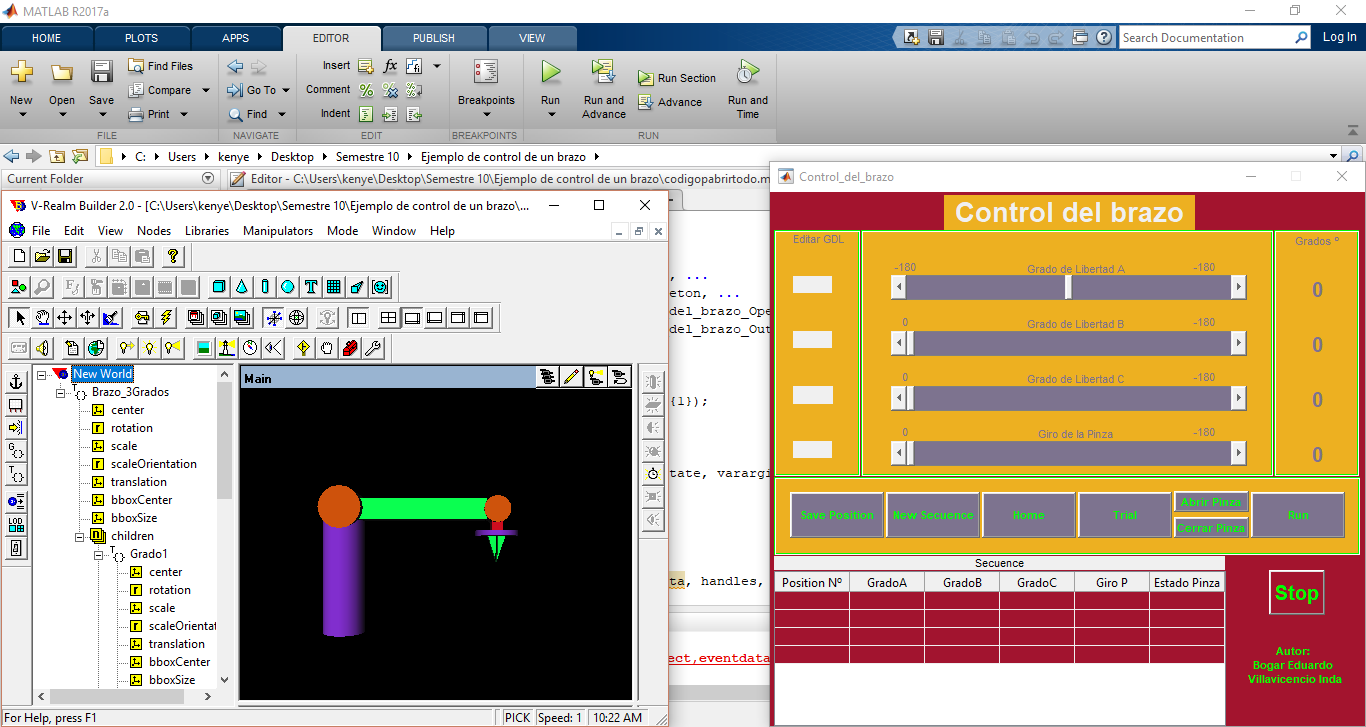
\includegraphics[width=0.9\textwidth, height=0.35\textheight]{./figs/matlabescritorio}\\
\caption{panel de control y robot en 3D.}
\label{matlabescritorio}
\end{figure}
\renewcommand\thechapter{\Roman{chapter}}
\chapter{CONCLUSIONES} \label{ch:conclusiones} \thispagestyle{fancy}
\renewcommand\thechapter{\arabic{chapter}}
%%%%%%%%%%%%%%%%%%%%%%%%%%%%%%%%%%%%%%%%%%%%%%%%%%%%%%%%%%%%%%%%%%%%%%%%%%%%
En este trabajo de tesis no se logra terminar el simulador, pero se aprovecha el potencial que Matlab tiene, ya que no se había manejado anteriormente el programa para crear diseños virtuales. Como no se había utilizado no se conocían las funciones del todo y poco a poco se fueron viendo hasta lograr lo que se ve en los resultados, de igual forma falta integrar la programación para enlazar el panel con el manipulador y poder finalmente tener un simulador, para así poder compararlo con lo que se quiere llegar, que es similar pero en Java3D. Teniendo los cálculos en Matlab será mas fácil hacer la programación, estudiando la API de Java3D para ver el código de importación y tener control sobre las piezas diseñadas anteriormente en SolidWorks.\\

Este tipo de herramientas crean un impacto positivo ya que en los trabajos vistos dentro de la investigación son favorables y se espera llegar o superar esos resultados.\\

Lo interesante de este proyecto es que una vez terminado se le puede dar seguimiento ya que es  código abierto, en caso de querer añadir mas funciones será posible.
%%%%%%%%%%%%%%%%%%%%%%%%%%%%%%%%%%%%%%%%%%%%%%%%%%%%%%%%%%%%%%%%%%%%%%%%%%%%%%%%%%%%%%%%%%%%%%%%%%%%
\titleformat{\chapter}{\centering\normalfont\Large\bfseries}{\thechapter}{1em}{}
\addcontentsline{toc}{chapter}{BIBLIOGRAFÍA}
\bibliography{referencias}
\bibliographystyle{plain}
%%%%%%%%%%%%%%%%%%%%%%%%%%%%%%%%%%%%%%%%%%%%%%%%%%%%%%%%%%%%%%%%%%%%%%%%%%%%%%%%%%%%%%%%%%%%%%%%%%%%
\appendix
\chapter{Quanser IP02} \label{apx:quanser}
%%%%%%%%%%%%%%%%%%%%%%%%%%%%%%%%%%%%%%%%%%%%%%%%%%%%%%%%%%%%%%%%%%%%%%%%%%%%

\begin{figure}
\centering

\includegraphics[width=8cm,height=5cm]{./figs/logoclr}
\caption{Logotipo del ITSON}
\end{figure}


\begin{table}
\centering
\begin{tabular}{clll}
\hline
Constante & Descripción & Valor & Unidades \\
\hline
$M$ & Masa del carro & 0.52 & kg \\
$B$ & Amortiguamiento viscoso & 0.9 & N$\cdot$ s/m \\
$K$ & RÍgidez del resorte & 160 & N/m \\
$\eta_g$ & Eficiencia de engranes & 1 & \\
$\eta_m$ & Eficiencia del motor & 1 & \\
$K_g$ & Relación de transmisión & 3.71 &  \\
$K_t$ & Constante de par & 0.00767 & N$\cdot$m/A \\
$K_m$ & Constante de fuerza magnetomotriz & 0.00767 & V$\cdot$s/rad \\ 
$R_m$ & Resistencia de armadura & 2.6 & $\Omega$ \\
$r_p$ & Radio pión & 6.35$\times$10$^{-3}$ & m \\
\hline
\end{tabular}
\caption{Parámetros del sistema Quanser. \label{tab:parametros}}
\end{table}
\end{document}